\documentclass[../teoria.root.tex]{subfiles}

\begin{document}

\section{Vectores}

Un vector es básicamente una flecha en el espacio. Esta flecha tiene un origen
y un extremo. Un vector que va del punto $A$ al punto $B$ se escribe
$\vec{AB}$:
\begin{center}
	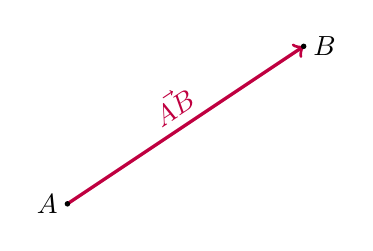
\begin{tikzpicture}
		\coordinate (a) at (1,1);
		\coordinate (b) at (4,3);
		\draw[->,very thick,purple] (a) -- (b) node[sloped,midway,above]{$\vec{AB}$};
		\fill (a) circle(1pt) node[left]{$A$};
		\fill (b) circle(1pt) node[right]{$B$};
	\end{tikzpicture}
\end{center}

Cabe aclarar que los vectores existen en todos los espacios, ya sea
$\mathbb{R}$, $\mathbb{R}^2$, $\mathbb{R}^3$, e incluso mayores dimensiones:

\begin{center}
	\begin{tikzpicture}[tdplot_main_coords]
		\draw[->] (0,0,0) -- (5,0,0) node[right]{$x$};
		\draw[->] (0,0,0) -- (0,5,0) node[above right]{$y$};
		\draw[->] (0,0,0) -- (0,0,4) node[above]{$z$};
		\draw[thick,dashed,xa] (0,3,0) -- (4,3,0);
		\draw[thick,dashed,ya] (4,0,0) -- (4,3,0);
		\draw[thick,dashed,za] (4,3,0) -- (4,3,3);
		\draw[thick,dashed,xa] (0,1,0) -- (2,1,0);
		\draw[thick,dashed,ya] (2,0,0) -- (2,1,0);
		\draw[thick,dashed,za] (2,1,0) -- (2,1,1);
		\draw[->,very thick,purple] (2,1,1) -- (4,3,3) node[midway,sloped,above]{$\vec{AB}$};
		\fill (2,1,1) circle(1pt) node[above left]{$A$};
		\fill (4,3,3) circle(1pt) node[above]{$B$};
	\end{tikzpicture}
\end{center}

\subsection{Vectores en el origen}

Cuando el origen del vector coincide con el origen del plano, este se puede
describir con solo el punto de su extremo:
\begin{center}
	\begin{tikzpicture}
		\pgfmathsetmacro{\x}{3}
		\pgfmathsetmacro{\y}{2}
		\draw[help lines] (-1,-1) grid (4,3);
		\draw[->] (-1,0) -- (4,0) node[right]{$x$};
		\draw[->] (0,-1) -- (0,3) node[above]{$y$};
		\draw[xa,thick] (0,0) -- (\x,0) node[midway,below]{$\x$};
		\draw[ya,thick] (\x,0) -- (\x,\y) node[midway,right]{$\y$};
		\draw[->,purple,very thick] (0,0) -- ++(\x,\y) node[midway,sloped,above]{$\vec{v}=(\x,\y)$};
	\end{tikzpicture}
\end{center}

Lo único que nos importa de un vector es su dirección y longitud, así que dos
vectores con orígenes y extremos distintos, mientras tengan la misma dirección
y longitud, son \textit{equivalentes}.

Para transformar un vector $\vec{AB}$ a un vector equivalente en el origen se
hace $\vec{OB}-\vec{OA}$ ($O$ siendo el origen del espacio):
\begin{center}
	\begin{tikzpicture}
		\coordinate (a) at (1,2);
		\coordinate (b) at (4,1);
		\draw[help lines] (-1,-2) grid (5,3);
		\draw[->] (-1,0) -- (5,0) node[right]{$x$};
		\draw[->] (0,-2) -- (0,3) node[above]{$y$};
		\draw[->,very thick,purple] (a) -- (b) node[midway,sloped,above]{$\vec{AB}$};
		\draw[->,very thick,blue] (0,0) -- (a) node[midway,sloped,above]{$\vec{OA}$};
		\draw[very thick,red,dashed] (0,0) -- (b) node[midway,sloped,above]{$\vec{OB}$};
		\draw[->,blue,very thick,dashed] (b) -- ($(b)-(a)$) node[midway,sloped,below]{$-\vec{OA}$};
		\draw[->, very thick,purple] (0,0) -- ($(b)-(a)$) node[midway,sloped,below]{$\vec{OB}-\vec{OA}$};
		\fill (a) circle(1pt) node[above]{$A$};
		\fill (b) circle(1pt) node[above]{$B$};
	\end{tikzpicture}
\end{center}

En la mayoría de los casos vamos a trabajar con vectores que empiezan en el
origen, ya que solo se requiere un punto para describirlos y son mas fáciles de
manipular.

\subsection{Suma}

Dos vectores se pueden sumar geométricamente colocando el origen de uno en el
extremo del otro. El vector que pasa por el origen del primero y el extremo del
ultimo es la suma de los vectores:
\begin{center}
	\begin{tikzpicture}
		\coordinate (v) at (3,1);
		\coordinate (w) at (1,2);
		\draw[->,very thick,blue] (0,0) -- ++(v) node[midway,sloped,below]{$\vec{v}$};
		\draw[->,very thick,purple] (v) -- ++(w) node[midway,sloped,below]{$\vec{w}$};
		\draw[->,very thick,green] (0,0) -- ++($(v)+(w)$) node[midway,sloped,above]{$\vec{v}+\vec{w}$};
		\draw[thick,blue,dashed] (w) -- ++(v);
		\draw[thick,purple,dashed] (0,0) -- ++(w);
	\end{tikzpicture}
\end{center}

Matemáticamente, La suma de dos vectores es sencillamente la suma de sus
componentes:
\[(x_1,y_1)+(x_2,y_2)=(x_1+x_2,y_1+y_2)\]

\subsection{Producto Por Escalar}

Un vector puede ser multiplicado por un numero (un escalar). Geométricamente,
esto es equivalente a escalar (de ahí el nombre) la magnitud de la flecha.
\begin{center}
	\begin{tikzpicture}
		\coordinate (v) at (2,.5);
		\draw[->,thick,green] (0,0) -- ++($2*(v)$) node[above]{$2\vec{v}$};
		\draw[->,thick,green] (0,0) -- ++($-1*(v)$) node[above]{$-\vec{v}$};
		\draw[->,very thick,blue] (0,0) -- ++(v) node[above]{$\vec{v}$};
	\end{tikzpicture}
\end{center}

Matemáticamente, lo único que hay que hacer es multiplicar cada componente del
vector por el escalar:
\[k(x,y)=(kx,ky)\]

\subsubsection{Vectores Paralelos}

Una propiedad importante de esta operación es que cualquier producto de un
vector por un escalar va a ser paralelo al vector original. Esto nos provee una
herramienta para determinar si dos vectores son paralelos:
\[\vec{v}\parallel\vec{w}\iff\exists k\in\mathbb{R}-\{0\}:k\vec{v}=\vec{w}\]

Dos vectores $\vec{v}$ y $\vec{w}$ son paralelos solo si existe un numero real
$k$ (que no sea $0$) tal que $k\vec{v}=\vec{w}$.

\subsection{Norma}

En $\mathbb{R}^2$, la longitud o norma de un vector $\vec{v}$, $\|\vec{v}\|$ se
puede conseguir utilizando el teorema de Pitágoras:
\begin{center}
	\begin{tikzpicture}
		\pgfmathsetmacro{\x}{3}
		\pgfmathsetmacro{\y}{2}
		\draw[help lines] (-1,-1) grid (4,3);
		\draw[->] (-1,0) -- (4,0) node[right]{$x$};
		\draw[->] (0,-1) -- (0,3) node[above]{$y$};
		\draw[xa,thick] (0,0) -- (\x,0) node[midway,below]{$x$};
		\draw[ya,thick] (\x,0) -- (\x,\y) node[midway,right]{$y$};
		\draw[->,purple,very thick] (0,0) -- ++(\x,\y) node[midway,sloped,above]{$\|\vec{v}\|=\sqrt{x^2+y^2}$};
	\end{tikzpicture}
\end{center}

Generalizando a otras dimensiones, la norma de un vector es la raíz cuadrada de
la suma de los cuadrados de sus componentes:
\[\|(x,y,z,\cdots)\|=\sqrt{x^2+y^2+z^2+\cdots}\]

Es interesante aclarar que el caso de una dimensión se reduce a calcular el
valor absoluto de un numero:
\[|x|=\sqrt{x^2}\]

\subsection{Producto Interno}

El producto interno de dos vectores es el producto de la norma del primer
vector por la norma de la proyección del segundo sobre el primero:

\begin{center}
	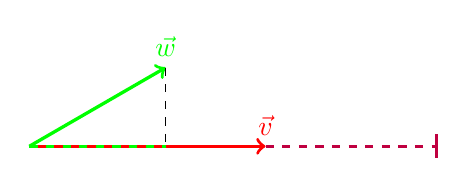
\begin{tikzpicture}
		\pgfmathsetmacro{\a}{30};
		\pgfmathsetmacro{\rw}{2};
		\pgfmathsetmacro{\rv}{3};
		\pgfmathsetmacro{\rp}{cos(\a)*\rw};
		\draw[-|,dashed,very thick,purple] (0:\rv) -- (0:\rp*\rv);
		\draw[->,very thick,red] (0,0) -- (0:\rv) node[above]{$\vec{v}$};
		\draw[->,very thick,green] (0,0) -- (\a:\rw) node[above]{$\vec{w}$};
		\draw[very thick,dashed,green] (0,0) -- (0:\rp);
		\draw[dashed] (\a:\rw) -- (0:\rp);
	\end{tikzpicture}
\end{center}

Esto se escribiría matemáticamente así:
\[\vec{v}\cdot\vec{w}=\|\vec{v}\|\|\vec{w}\|\cos\theta\]

Por suerte, hay una cuenta mucho mas fácil: El producto interno de dos vectores
se consigue sumando los productos de los componentes de los vectores:
\[(x_1,y_1)\cdot(x_2,y_2)=x_1x_2+y_1y_2\]

Es difícil explicar el producto interno de forma intuitiva, así que los derivo
en este caso a \eola, que da una explicación geométrica muy intuitiva
utilizando transformaciones lineales.

\subsubsection{Vectores Perpendiculares}

Una propiedad importante del producto interno es que ya que depende del coseno
del angulo entre los dos vectores, si los vectores son perpendiculares (su
angulo es \ang{90}) su producto interno va a ser $0$. (ya que
$\cos\ang{90}=0$).
\[\vec{v}\perp\vec{w}\iff\vec{v}\cdot\vec{w}=0\]

En $\mathbb{R}^2$, dado un vector $\vec{v}$, una solución general a la ecuación
$\vec{v}\cdot\vec{w}=0$ es $\vec{v}=(w_y,-w_x)$. Por ejemplo, para encontrar un
vector perpendicular a $(2,3)$:
\begin{align*}
	\vec{v}\perp(2,3)\iff\vec{v}\cdot(2,3)&=0\\
	\vec{v}&=(3,-2)\\
	2v_x+3v_y&=0\\
	2\cdot3+3\cdot-2&=0\\
	6-6&=0\\
	0&=0
\end{align*}

\subsubsection{Ángulo entre vectores}

Ya que el producto interno se puede determinar con dos cuentas distintas, y una
utiliza el angulo entre los vectores, estas se pueden combinar para conseguir
una ecuación para conseguir el angulo entre dos vectores:
\[\vec{v}\cdot\vec{w}=\|\vec{v}\|\|\vec{w}\|\cos\theta\]
\[\cos\theta=\frac{\vec{v}\cdot\vec{w}}{\|\vec{v}\|\|\vec{w}\|}\]
\[\theta=\cos^{-1}\frac{\vec{v}\cdot\vec{w}}{\|\vec{v}\|\|\vec{w}\|}\]

\subsection{Producto Vectorial}

En espacios $\mathbb{R}^3$, existe otra operación que se puede hacer entre
vectores: El producto vectorial.

Geométricamente, el producto vectorial de dos vectores va a ser otro vector,
perpendicular a ambos. Su magnitud seria el determinante de una matriz formada
por los vectores (un tema que veremos a fondo mas adelante).

El producto vectorial \textbf{no es conmutativo},
$\vec{v}\times\vec{w}\neq\vec{w}\times\vec{v}$, los vectores resultantes van a
ser iguales, pero van a ir en direcciones opuestas:
\[\vec{v}\times\vec{w}=-(\vec{w}\times\vec{v})\]

\begin{center}
	\begin{tikzpicture}[tdplot_main_coords]
		\draw (-3,0,0) -- (3,0,0);
		\draw (0,-3,0) -- (0,3,0);
		\draw (0,0,-3) -- (0,0,3);
		\draw[->,very thick,red] (0,0) -- (1,0,0) node[below]{$\vec{v}$};
		\draw[->,very thick,blue] (0,0) -- (0,2,0) node[right]{$\vec{w}$};
		\draw[->,very thick,purple] (0,0) -- (0,0,2) node[above left]{$\vec{v}\times\vec{w}$};
		\draw[->,very thick,purple] (0,0) -- (0,0,-2) node[below left]{$\vec{w}\times\vec{v}$};
	\end{tikzpicture}
\end{center}

Matemáticamente, la cuenta seria:
\[\begin{pmatrix}\vx\\\vy\\\vz\end{pmatrix}\times
\begin{pmatrix}\wx\\\wy\\\wz\end{pmatrix}=
\begin{pmatrix}
	\vy\wz-\vz\wy\\
	\vz\wx-\vx\wz\\
	\vx\wy-\vy\wx
\end{pmatrix}\]

Esta cuenta no es precisamente intuitiva, y los derivo nuevamente a \eola, que
da una buena explicación. Como ayuda para memorizar, el valor de cada fila se
puede ver como una especie de producto cruzado entre las filas que quedan al
eliminar la fila en cuestión:
\[\begin{pmatrix}\transparent{0.2}\vx\\\vy\\\vz\end{pmatrix}\times
\begin{pmatrix}\transparent{0.2}\wx\\\wy\\\wz\end{pmatrix}=
\begin{pmatrix}
	\vy\wz-\vz\wy\\
	\transparent{0.2}\vz\wx-\vx\wz\\
	\transparent{0.2}\vx\wy-\vy\wx
\end{pmatrix}\]
\[\begin{pmatrix}\vx\\\transparent{0.2}\vy\\\vz\end{pmatrix}\times
\begin{pmatrix}\wx\\\transparent{0.2}\wy\\\wz\end{pmatrix}=
\begin{pmatrix}
	\transparent{0.2}\vy\wz-\vz\wy\\
	\vz\wx-\vx\wz\\
	\transparent{0.2}\vx\wy-\vy\wx
\end{pmatrix}\]
\[\begin{pmatrix}\vx\\\vy\\\transparent{0.2}\vz\end{pmatrix}\times
\begin{pmatrix}\wx\\\wy\\\transparent{0.2}\wz\end{pmatrix}=
\begin{pmatrix}
	\transparent{0.2}\vy\wz-\vz\wy\\
	\transparent{0.2}\vz\wx-\vx\wz\\
	\vx\wy-\vy\wx
\end{pmatrix}\]

Cuando veamos el tema de los determinantes, esta cuenta va a ser mucho mas
clara.

\subsubsection{Regla de la mano derecha}

Una forma de memorizar la dirección del vector resultante de un producto
vectorial es con la regla de la mano derecha. Primero se extiende el dedo
índice hacia adelante y el pulgar hacia arriba, como una pistola, y el medio se
extiende perpendicular a los anteriores. Imaginando a los vectores $\vec{v}$ y
$\vec{w}$ como los dedos indice y medio, la dirección del vector
$\vec{v}\times\vec{w}$ va a ser la del pulgar.

\end{document}
